\subsection{Simulation}
\label{sec:results}

When software development was nearing completion, the project's hypotheses
could be tested. This section will describe how that was done, starting with
explaining how the simulation was set up in Section \ref{sec:results:inputs}.
Simulation results are discussed in Section \ref{sec:results:profits}, with an
in-depth look at the performance of the Q-Learner in Section
\ref{sec:results:ai}. Finally, the results are reviewed in Section
\ref{sec:results:summary}.


\subsubsection{Inputs}
\label{sec:results:inputs}

The experiments and their analysis can be repeated by using Taxi-sim and
following the instructions in User Manual in Appendix \ref{sec:user_manual}.
The result datasets can be found in the open data set mentioned in
\ref{sec:intro:overview}.

Initially a baseline of inputs were chosen without any intentional constraints
on the environmental conditions. These inputs are shown in Table
\ref{table:input_data} and the full result data can be found in
\texttt{standard} directory in the data set.

\begin{table}
\begin{tabular}{ | l | l | }
  \hline
  Parameter & Value \\ \hline
  Time Limit & 1 000 000 \\
  Road network & as in Figure \ref{figure:results:road_network} \\
  Passengers' expected fare & 20 \\
  Q-Learner's greediness \(\varepsilon\) & 0.9 \\
  Q-Learner's discount factor \(\gamma\) & 0.9 \\
  Q-Learner's default value estimate & 0 \\
  Taxi's variable price range & 5-100 (integers) \\
  Taxi's benchmark price & 20 \\
  \hline
\end{tabular}
\caption{
  Simulation inputs
  \label{table:input_data}
}
\end{table}

\begin{figure}
\begin{center}
  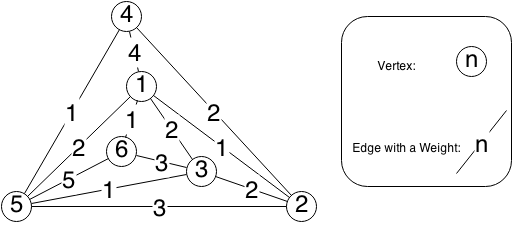
\includegraphics[width=\textwidth]{../figures/road_network}
  \caption{
    Simulation's Input Road Network
    \label{figure:results:road_network}
  }
\end{center}
\end{figure}

The simulation was additionally run for control purposes, varying one input
parameter at a time. These runs are summarised in Table
\ref{table:inputs:control}, displaying the parameter in question and its
changed value, as well as the directory in the open data source where the
results are located.

\begin{table}
\begin{tabular}{ | l | l | l | }
  \hline
  Parameter & Value & Result Directory \\ \hline
  No changes & - & \texttt{standard} \\
  Benchmark price & 15 & \texttt{lower\_benchmark} \\
  Benchmark price & 30 & \texttt{higher\_benchmark} \\
  Q-Learner's default value estimate & 10 & \texttt{value\_estimate\_10} \\
  Q-Learner's default value estimate & 100 & \texttt{value\_estimate\_100} \\
  Q-Learner's default value estimate & -10 & \texttt{value\_estimate\_neg10} \\
  Q-Learner's default value estimate & -100 & \texttt{value\_estimate\_neg100} \\
  Q-Learner's discount factor & 0.4 & \texttt{lower\_discount} \\
  Q-Learner's greediness & 0.4 & \texttt{lower\_greediness} \\
  Taxi's price range & 5 - 20 & \texttt{lower\_range} \\
  Taxi's price range & 20 - 100 & \texttt{higher\_range} \\
  Time limit & 50 000 & \texttt{limited\_time} \\
  \hline
\end{tabular}
\caption{
  Control parameter changes
  \label{table:inputs:control}
}
\end{table}

Besides the configurable inputs, some simulation parameters used defaults
fixed in the source code. Passenger characteristics were manually adjusted so
that the probability of a passenger accepting a fare would be about 75\% for
their expected fare, as in preceding test simulation runs it was experimentally
determined that the formula in Section \ref{sec:requirements:passenger}
resulted in this probability being lower than 10\%.


\subsubsection{Profitability}
\label{sec:results:profits}

Full results and a detailed simulation analysis can be found included in the
project's data set at the web address specified in Section
\ref{sec:intro:online}. This data is organised by simulation runs as identified
in Table \ref{table:inputs:control}, and each simulation run has two parts -- variable
pricing and benchmark.

Before any result analysis is started, it is important to remember that these
results are relative and should be treated as such. Even though the data has
exact numbers, they have no basis in reality. For example, the agents could
have made a loss in all simulations had the taxi costs been set greater.

In all simulation runs, the variable pricing approach performed significantly
better. The summary of total profits are shown in Figure
\ref{figure:results:total_profit}, ordered descending from left to right by
total profit in the simulation using variable fares.

\begin{figure}
\begin{center}
  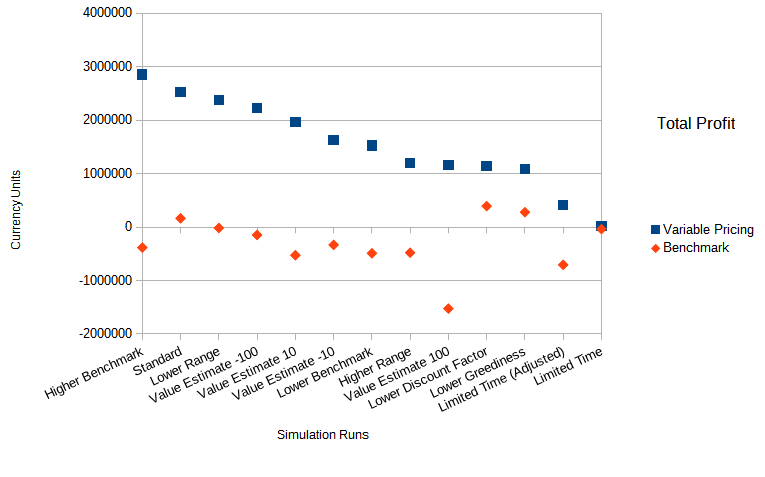
\includegraphics[width=\textwidth]{../figures/total_profit}
  \caption{
    Summary of Total Profits in Simulation Results
    \label{figure:results:total_profit}
  }
\end{center}
\end{figure}

The most profitable simulation runs were the runs with a higher fixed benchmark
price and the run with default settings. The worst performance (when adjusted
for the same timescale) was shown by the simulation with a limited timeframe,
which most likely did not have sufficient time to find a near-optimal policy.

Interestingly, the third most profitable was the simulation where the agent was
limited to a price range lower than the passenger's expected fare and lower
than its corresponding fixed benchmark price. This beyond doubt proves that a
flexible approach is more profitable than sticking to a fixed fare price
structure. However, the simulation with a higher variable price range seems to
have performed badly compared to the lower price range, although it is still
much more profitable than the benchmark simulation.

The effect of initial value estimates on the learner seems to have an important
role when they are significantly overvalued. The simulation run 'Value Estimate
100' when comparing the variable price results fared almost as badly as the
simulations with lowered discount factor and greediness that are impaired in
turn by overly focusing on current rewards and by selecting a random action
very often. Additionally the overvalued estimates resulted in an exceptionally
low profit for the fixed price simulation. However, when the value estimates
were close to the actual estimates or significantly undervalued, the simulation
results show only small performance differences that could easily be explained
by randomness.

Nevertheless, these results strongly suggest that in identical conditions
having a choice to charge a varied range of fare prices is advantageous to a
taxi's profitability, and that Q-Learning can successfully be used for setting
the fare prices.


\subsubsection{Performance of Reinforcement Learning}
\label{sec:results:ai}

Analysis of variance was performed on each simulation's dataset (meaning that
benchmark and variable pricing runs were analysed separately), and linear
regression of reinforcement learning agent's observed rewards performed. The
full results are available at the web address specified in Section
\ref{sec:intro:online}. The following results have a 95\% confidence rate
unless mentioned otherwise.

All bar one of the simulation runs show an increase of rewards over time for
variable pricing taxi agents. These reward regressions are shown in Figure
\ref{figure:results:variable_rewards}. The agent in the simulation run with a
lower range of prices might have settled on a sub- optimal policy for a large
part of its lifetime, hence the trend of decreasing reward.

\begin{figure}
\begin{center}
  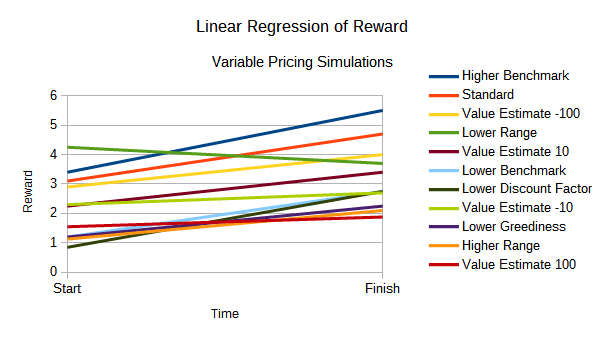
\includegraphics[width=\textwidth]{../figures/reward_regression_variable}
  \caption{
    Regression Analysis of Rewards (Variable Pricing)
    \label{figure:results:variable_rewards}
  }
\end{center}
\end{figure}

Data runs with a fixed price paint a similar picture (see Figure
\ref{figure:results:fixed_rewards}) with most agents steadily increasing their
rewards. However, there is an outlier here as well: the simulation with a
considerably overvalued initial value estimate failed to make any statistically
significant change to their average reward over the course of the simulation.
Unsurprisingly, this was the least profitable simulation with a fixed price as
can be seen in \ref{figure:results:total_profit} and is described in Section
\ref{sec:results:profits}.

\begin{figure}
\begin{center}
  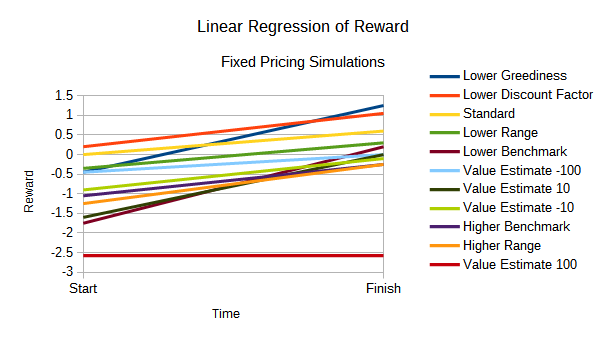
\includegraphics[width=\textwidth]{../figures/reward_regression_fixed}
  \caption{
    Regression Analysis of Rewards (Fixed Pricing)
    \label{figure:results:fixed_rewards}
  }
\end{center}
\end{figure}

\subsubsection{Summary}
\label{sec:results:summary}

To conclude, the results suggest that the taxi agent was successful at finding
a policy that increases the average reward when it can choose the price freely.
However, the results clearly reveal the importance of setting the environmental
conditions and constraints, which can have a large influence on the
effectiveness of the reinforcement learning.

Worryingly, there was a simulation where the agent showed no change in rewards.
This lack of change raises questions about the correctness of the software, as
the policy was clearly sub-optimal but the rewards did not change unlike in
other simulation runs. There is a possibility that this was caused by a design
oversight or even a bug in the implementation, although the remainder of the
runs seem to have been successful and correct.
